\documentclass[ngerman,a4paper,abstracton,open=right,twoside=false,toc=listofnumbered,bibtotocnumbered]{scrreprt}
\usepackage[utf8]{inputenc}
\usepackage[T1]{fontenc}
\usepackage{lmodern}
\usepackage{babel}
\usepackage{geometry}
\usepackage{graphicx}
\usepackage[hidelinks]{hyperref}
\usepackage{listings}
\usepackage{color}
\usepackage[scaled=.8]{beramono}
\geometry{a4paper, top=20mm, bottom=40mm, left=40mm, right=25mm, footskip=20mm}

\lstdefinelanguage{clojure}
{morekeywords={*,*1,*2,*3,*agent*,*allow-unresolved-vars*,*assert*,*clojure-version*,*command-line-args*,
*compile-files*,*compile-path*,*e,*err*,*file*,*flush-on-newline*,*in*,*macro-meta*,
*math-context*,*ns*,*out*,*print-dup*,*print-length*,*print-level*,*print-meta*,*print-readably*,
*read-eval*,*source-path*,*use-context-classloader*,*warn-on-reflection*,+,-,->,->>,..,/,:else,
<,<=,=,==,>,>=,@,accessor,aclone,add-classpath,add-watch,agent,agent-errors,aget,alength,alias,
all-ns,alter,alter-meta!,alter-var-root,amap,ancestors,and,apply,areduce,array-map,aset,
aset-boolean,aset-byte,aset-char,aset-double,aset-float,aset-int,aset-long,aset-short,assert,
assoc,assoc!,assoc-in,associative?,atom,await,await-for,await1,bases,bean,bigdec,bigint,binding,
bit-and,bit-and-not,bit-clear,bit-flip,bit-not,bit-or,bit-set,bit-shift-left,bit-shift-right,
bit-test,bit-xor,boolean,boolean-array,booleans,bound-fn,bound-fn*,butlast,byte,byte-array,
bytes,cast,char,char-array,char-escape-string,char-name-string,char?,chars,chunk,chunk-append,
chunk-buffer,chunk-cons,chunk-first,chunk-next,chunk-rest,chunked-seq?,class,class?,
clear-agent-errors,clojure-version,coll?,comment,commute,comp,comparator,compare,compare-and-set!,
compile,complement,concat,cond,condp,conj,conj!,cons,constantly,construct-proxy,contains?,count,
counted?,create-ns,create-struct,cycle,dec,decimal?,declare,def,definline,defmacro,defmethod,
defmulti,defn,defn-,defonce,defprotocol,defstruct,deftype,delay,delay?,deliver,deref,derive,
descendants,destructure,disj,disj!,dissoc,dissoc!,distinct,distinct?,do,do-template,doall,doc,
dorun,doseq,dosync,dotimes,doto,double,double-array,doubles,drop,drop-last,drop-while,empty,empty?,
ensure,enumeration-seq,eval,even?,every?,false,false?,ffirst,file-seq,filter,finally,find,find-doc,
find-ns,find-var,first,float,float-array,float?,floats,flush,fn,fn?,fnext,for,force,format,future,
future-call,future-cancel,future-cancelled?,future-done?,future?,gen-class,gen-interface,gensym,
get,get-in,get-method,get-proxy-class,get-thread-bindings,get-validator,hash,hash-map,hash-set,
identical?,identity,if,if-let,if-not,ifn?,import,in-ns,inc,init-proxy,instance?,int,int-array,
integer?,interleave,intern,interpose,into,into-array,ints,io!,isa?,iterate,iterator-seq,juxt,
key,keys,keyword,keyword?,last,lazy-cat,lazy-seq,let,letfn,line-seq,list,list*,list?,load,load-file,
load-reader,load-string,loaded-libs,locking,long,long-array,longs,loop,macroexpand,macroexpand-1,
make-array,make-hierarchy,map,map?,mapcat,max,max-key,memfn,memoize,merge,merge-with,meta,
method-sig,methods,min,min-key,mod,monitor-enter,monitor-exit,name,namespace,neg?,new,newline,
next,nfirst,nil,nil?,nnext,not,not-any?,not-empty,not-every?,not=,ns,ns-aliases,ns-imports,
ns-interns,ns-map,ns-name,ns-publics,ns-refers,ns-resolve,ns-unalias,ns-unmap,nth,nthnext,num,
number?,odd?,or,parents,partial,partition,pcalls,peek,persistent!,pmap,pop,pop!,pop-thread-bindings,
pos?,pr,pr-str,prefer-method,prefers,primitives-classnames,print,print-ctor,print-doc,print-dup,
print-method,print-namespace-doc,print-simple,print-special-doc,print-str,printf,println,println-str,
prn,prn-str,promise,proxy,proxy-call-with-super,proxy-mappings,proxy-name,proxy-super,
push-thread-bindings,pvalues,quot,rand,rand-int,range,ratio?,rational?,rationalize,re-find,
re-groups,re-matcher,re-matches,re-pattern,re-seq,read,read-line,read-string,recur,reduce,ref,
ref-history-count,ref-max-history,ref-min-history,ref-set,refer,refer-clojure,reify,
release-pending-sends,rem,remove,remove-method,remove-ns,remove-watch,repeat,repeatedly,
replace,replicate,require,reset!,reset-meta!,resolve,rest,resultset-seq,reverse,reversible?,
rseq,rsubseq,second,select-keys,send,send-off,seq,seq?,seque,sequence,sequential?,set,set!,
set-validator!,set?,short,short-array,shorts,shutdown-agents,slurp,some,sort,sort-by,sorted-map,
sorted-map-by,sorted-set,sorted-set-by,sorted?,special-form-anchor,special-symbol?,split-at,
split-with,str,stream?,string?,struct,struct-map,subs,subseq,subvec,supers,swap!,symbol,symbol?,
sync,syntax-symbol-anchor,take,take-last,take-nth,take-while,test,the-ns,throw,time,to-array,
to-array-2d,trampoline,transient,tree-seq,true,true?,try,type,unchecked-add,unchecked-dec,
unchecked-divide,unchecked-inc,unchecked-multiply,unchecked-negate,unchecked-remainder,
unchecked-subtract,underive,unquote,unquote-splicing,update-in,update-proxy,use,val,vals,
var,var-get,var-set,var?,vary-meta,vec,vector,vector?,when,when-first,when-let,when-not,
while,with-bindings,with-bindings*,with-in-str,with-loading-context,with-local-vars,
with-meta,with-open,with-out-str,with-precision,xml-seq,zero?,zipma
},
   sensitive,
   alsodigit=-,
   morecomment=[l];,
   morestring=[b]"
  }[keywords,comments,strings]

\definecolor{forkeywords}{rgb}{0.5,0.0,0.33}

\lstset{
	language=clojure,
	basicstyle=\ttfamily,
	keywordstyle=\bfseries\color{forkeywords},
	showstringspaces=false,
	frame=single,
	breaklines=true}

\title{Leistungsvergleich von Clojure--Parsern}
\subtitle{Technischer Bericht zum Masterprojekt}
\author{Daniel Kirsten (daniel.kirsten@mni.thm.de)
\and
Markus Bader (markus.bader@mni.thm.de)
\and\\
\emph{betreut durch Prof. Dr. B. Renz (burkhardt.renz@mni.thm.de)}
}
\publishers{Technische Hochschule Mittelhessen, Fachbereich MNI, Wiesentraße 14, D--35390 Gießen}

\date{\today}
\begin{document}

\maketitle
\newpage
\begin{abstract}

Im Rahmen des Masterprojekts im Wintersemester 2013/2014 haben die Autoren ein Programm zum Anwenden von Logikfunktionen (z. B. Wahrheitstafeln, Tseitin--Transformation, SAT--Solving) entworfen und mittels der Programmiersprache Clojure implementiert. Unter anderem wird ein Parser zum Umwandeln von logischen Formeln in eine Clojure--Datenstruktur benötigt.

Zu diesem Zweck wurde ein Parser mittels der Bilbiothek Instaparse erzeugt, jedoch viel dessen signifkant längere Laufzeit gegenüber einem JavaCC--Vergleichsparser auf.

In diesem technischen Bericht, welcher zugleich die Abschlussdokumentation zum Projekt darstellt, werden die Laufzeiten von fünf Parsern verglichen: Instaparse und Kern, jeweils mit einer vollständigen und einer minimierten Grammatik, sowie der JavaCC--Referenzparser.

\end{abstract}
\newpage
\tableofcontents
\newpage

\chapter{Einführung}

Bevor auf die eigentlichen Messungen eingegangen wird, sollen zunächst diverse Hintergrundinformationen zu dem Projekt sowie den Parser--Bibliotheken gegeben werden.

\section{MPA}

Der \emph{MNI Proposition Analyzer (MPA)} ist ein im Institut für Softwarearchitektur (ISA) des Fachbereichs Mathematik, Naturwissenschaften und Informatik (MNI) an der Technischen Hochschule Mittelhessen (THM) entwickeltes Programm, um übliche Berechnungen im Bereich der Aussagenlogik anzuwenden. \cite{mpa}

Zu den Features gehören u. a.:

\begin{itemize}
	\item Parsen von Formeln
	\item Ausgeben einer Wahrheitstabelle
	\item Produktion der konjunktiven und disjunktiven Normalform (CNF, DNF)
	\item Anwenden der Tseitin--Transformation
	\item Überprüfen der Erfüllbarkeit einer Formel mittels eines externen SAT--Solver (z. B. SAT4J)
	\item Pretty--print--Funktionen z. B. für Tex.
	\item Anwenden eines externen, M4--kompatiblen Makroprozessors
\end{itemize}

Die Funktionen können über Kommandozeile oder eine GUI angesprochen werden. Das Programm wird in der Lehre an der THM eingesetzt und ist unter der GPL quelloffen verfügbar.

\section{Logical Workbench}

Innerhalb des Masterprojektes der Autoren unter Leitung des bereits für den MPA verantwortlichen Prof. Dr. B. Renz wird ein Programm mit identischen oder ähnlichen Funktionen des MPA entwickelt. Unter dem Projektnamen \emph{Logical Workbench (LW)} wird im Gegensatz zu Java jedoch die Programmiersprache \emph{Clojure} verwendet.

Clojure ist ein LISP, welches zu Java--Bytecode kompiliert wird und somit auf der JVM arbeitet. Als Besonderheit ist die einfache Verwendung von Java--Code (etwa Klassen) zu nennen, wodurch auch ein von JavaCC generierter Parser--Code benutzt werden kann (siehe Abschnitt \ref{JavaCC}).

Zum Zeitpunkt des Verfassens dieses Textes sind die Kernfunktionen implementiert; im Einzelnen:

\begin{itemize}
	\item Parsen von Formeln
	\item Ausgeben einer Wahrheitstabelle
	\item Produktion der CNF (mittels trivialem Algorithmus oder Tseitin--Transformation)
	\item Generieren des Dimacs--Formats und Aufrufen von SAT4J
\end{itemize}

Ein Makroprozessor wurde nicht eingebunden, da Clojure selbst über ein mächtiges Makrosystem verfügt. Im weiteren Verlauf des Projektes sind die Implementierung einer dem MPA ähnlichen GUI und ein System zum Anwenden der natürlichen Deduktion geplant. Der Code des Projektes ist unter \cite{lw} einsehbar.

\section{Das Problem: Parser--Laufzeiten}

Zu der wesentlichen Kernfunktionalität der LW gehört das Parsen von Formeln, so dass eine Clojure--Liste entsteht, also beispielsweise der String \lstinline|"A -> !(A & B)"| zu \lstinline|(impl A (not (and A B)))| geparst wird. Die vollständige Referenzgrammatik des MPA findet sich in Anhang \ref{refgrammatik}.

Zunächst wurde zur allgemeinen Zufriedenheit die Bibliothek \emph{Instaparse} verwendet. Bei einem Test mit einer großen Formel (Sudoku--Regeln) wurde jedoch eine im Vergleich mit dem Referenzparser sehr viel höhere Laufzeit festgestellt, wenn der mit Instaparse generierte Parser nicht vorher durch einen Stackoverflow abgebrochen wurde. So brauchte dieser in einem Testdurchlauf mehrere Minuten, wogegen der Referenzparser des MPA diese Aufgabe in etwa zwei Sekunden vollbrachte.

Aus diesem Grunde wurden zunächst die Ursachen für die stark wachsende Laufzeit des Instaparse--Parsers eruiert und anschließend eine Vergleichsmessung zwischen verschiedenen Parsern und Grammatiken durchgeführt.

\section{Die Parser--Bibliotheken}

In diesem Abschnitt sollen die für den Vergleich benutzten Parser--Bibliotheken nicht nur vorgesellt werden, auch ihre Anwendung, Konzepte und Eigenheiten werden in Kürze umrissen.

\subsection{Instaparse}

Die von Mark Engelberg entwickelte Bibliothek \emph{Instaparse} gehört zur Gruppe der Parser--Generatoren, d. h. es wird eine Grammatik angegeben, aus der dann ein Programm generiert wird, welches eine Zeichenkette gemäß der Grammatik parsen kann. Da ein Clojure--Programm zur Laufzeit übersetzt werden kann, ist zur Verwendung des generierten Programms kein weiterer Kompilier--Zwischenschritt notwendig, wie etwa bei JavaCC. \cite{instaparse}

Instaparse ist komplett in Clojure geschrieben und wurde deswegen und aufgrund der Simplizität zunächst als Parser für die LW gewählt. So sehen die Schritte zur Entwicklung eines Parsers beispielhaft so aus:

\begin{enumerate}
	\item In einem Clojure--String oder einer externen Text--Datei wird eine Grammatik spezifiziert.
	\item Diese Grammatik wird als Argument einer Funktion \glqq{}parse\grqq{} verwendet, welche den Parser zurückgibt, z. B. \lstinline|(def logic-parser (insta/parser "src/logic/grammar.txt"))|.
	\item Mit diesem Parser kann ein String geparst werden, z. B. erzeugt \lstinline|(logic-parser "A & B")| einen abstrakten Syntaxbaum (AST) \lstinline|[:and [:atom "A"] [:atom "B"]]|. Als Ausgabeformat stehen dabei hiccup oder enlive zur Verfügung.
	\item Die Funktion \glqq{}transform\grqq{} nimmt einen AST und eine Hash--Map zur Substitution an und kann den Parsebaum somit umwandeln. Aus obigem AST wird somit etwa \lstinline|(and A B)|.
\end{enumerate}

\subsection{Kern}

Im Gegensatz zu JavaCC und Instaparse gehören mit \emph{Kern} geschriebene Parser zur Gruppe der Combinator--Parser. Dabei gibt es mehrere \glqq{}kleine\grqq{} Parser, also z. B. einen, der eine Konjunktion parst, und einen, der ein Atom parsen kann. Diese Einzelparser können dann mit sogenannten Kombinatoren miteinander verbunden werden, um einen größeren Parser zu erzeugen. Kern bietet eine Reihe von Funktionen, Makros und Datenstrukturen, um solche Combinator--Parser zu erzeugen, z.B. ChainL--Funktionen.

Im Gegensatz zu Instaparse verfügt es dabei über einen dedizierten Lexer, welcher sich nahtlos in die Parsergrammatik einfügt. Dies sorgt einerseits für kompakten Code, kann andererseits aber auch verwirren. So sind \lstinline|token*| und \lstinline|token_| Parser--Funktionen, \lstinline|token| jedoch eine Funktion des Lexers und verlangt einen solchen korrekt eingebunden und eingestellt. Dafür erhöht der Lexer die Komfortabilität, da z. B. die für einen Identifier erlaubten Zeichen als einfacher regulärer Ausdruck angegeben werden können und sich der Benutzer daraufhin nicht mehr um Leerzeichen kümmern muss.

Das Äquivalent zur benötigten Grammatik kann im Sourcecode unter \cite{lw} eingesehen werden. Zu Beachten ist, dass der Autor selber aussagt, dass seine Bibliothek nicht performant ist. 

\begin{quote}
	``Kern's design isn't well-suited for achieving very high performance.'' \cite{kern}
\end{quote}

\subsection{JavaCC}\label{JavaCC}

Wie Instaparse gehört \emph{JavaCC} zur Gruppe der Parser--Generatoren. Es ist jedoch eine Java--Bibliothek und schon weitaus länger in Entwicklung, so dass es ausgereifter ist. \cite{javacc}

JavaCC verlangt eine Grammatik, in der nicht nur die Parseregeln, sondern auch die Regeln des zu produzierenden Codes festgelegt werden können. Daraus erzeugt JavaCC dann Java--Code, der kompiliert dann als Parser verwendet werden kann. Da Clojure die Möglichkeit bietet, Java--Code direkt zu verwenden, kann der Quellcode des JavaCC aus dem MPA übernommen werden; es muss jedoch eine andere Ausgabe erzeugt werden. So besteht im MPA der AST aus verschiedenen Klassen des Types \glqq{}Knoten\grqq{} (Node) und kann unter Einsatz eines Visitor--Patterns transformiert werden. Um die in der LW verwendeten Clojure--Listen zu produzieren, wird mittels einer Funktion rekursiv durch den AST traversiert und die neue Struktur aus den Java--Klassen erzeugt.

Die Bibliothek stellt ebenfalls einen Lexer bereit, jedoch kann dieser nicht optional verwendet werden, sondern es müssen alle Token durch diesen erkannt und an den Parser weitergegeben werden können. JavaCC wird produktiv eingesetzt.

\chapter{Versuchsaufbau}

Da wie bereits erwähnt der zuerst implementierte Instaparse--Parser bei einem Beispiel nicht mehr verwendbar war, kam die Idee auf, verschiedene Parser zu vergleichen. Neben besagtem Instaparse und der JavaCC--Referenzimplementierung sollte noch ein Parser verglichen werden, der nach einem gänzlich anderem Prinzip arbeitet. Die Wahl fiel auf Kern.

Um die Ergebnisse der Laufzeitmessung vergleichbar und möglichst aussagekräftig zu halten, müssen die Rahmenbedingungen definiert werden. Dazu gehört die Auswahl der Formeln --- nach quantitativem und qualitativem Umfang, sowie eine bestimmte Reduktion der Grammatiken, um den Laufzeitunterschied mit einem Anwachsen der Parse--Regeln beurteilen zu können.

\section{Allgemeine Aspekte}

Die Messung wird mit der Methode \glqq{}time\grqq{} gemessen. Es zählt der Aufruf des Parsers und Zum Thema der Geschwindigkeit des Instaparse--Parsers hat sich der Autor von Instaparse ggf. das Anwenden einer Transformationsfunktion (um aus einem AST Clojure--Listen z
u machen), d. h. es wird immer mit der zu parsenden Formel aufgerufen und es wird letztendlich die selbe Clojure--Datenstruktur erzeugt. Innerhalb der Zeitmessung wird weder auf der Konsole ausgegeben (dies kann zusätzliche Zeit in Anspruch nehmen), noch sind sonstige Seiteneffekte zugelassen.

Sofern möglich, wird jede Formel mit jedem Parser und jeder der für ihn definierten Grammatiken aufgerufen. Ist dies in einem besonderen Fall nicht möglich, so kann ein errechneter Wert angegeben werden, insofern er als solcher markiert wird. Jeder so mögliche Durchlauf wird zehnmal ausgeführt und von allen Ergebnissen das arithmetische Mittel gebildet.

Da einige Parser ihren Zustand des letzten Aufrufes speichern können, ist bei mehreren gleichen Aufrufen hintereinander der erste Aufruf signifikant langsamer als die anderen. Aus diesem Grunde dürfen mit jeweils einem Parser keine zwei identischen Aufrufe direkt aufeinanderfolgend ausgeführt werden. Hierfür wurde für jeden Messdurchlauf die REPL neu gestartet.

\section{Grammatiken}

Als Referenz der zu enthaltenden Regeln dient die Parse--Grammatik des MPA (siehe Anhang \ref{refgrammatik}). Es wurden ähnliche Definitionen für Instaparse und Kern vorgenommen und sie produzieren zumindest für die Testformeln das gleiche Ergebnis. Diese Grammatiken werden im Folgenden \emph{volle Grammatiken} genannt.

Um jedoch das Wachstum der Laufzeit durch Hinzufügen von weiteren Regeln messen zu können, wurde für Kern und Instaparse jeweils eine weitere Grammatik definiert. Diese kann nur Formeln verarbeiten, welche enhalten:

\begin{itemize}
	\item Binäroperatoren \glqq{}and\grqq{} und \glqq{}or\grqq{} durch die Zeichen \glqq{}\&\grqq{} bzw. \glqq{}|\grqq
	\item Unäroperator \glqq{}not\grqq{} durch das Zeichen \glqq{}!\grqq
	\item Klammerung mit runden Klammern
	\item Atome, beginnend mit einem Kleinbuchstaben, fortführend mit Unterstrich, Kleinbuchstaben oder ganze Zahlen
\end{itemize}

Leerzeichen sind dabei nicht erlaubt. Diese Art von Grammatiken wird ab jetzt \emph{minimale Grammatik} genannt.

\section{Formeln}

Um aussagekräftige Messergebnisse zu erhalten, mussten repräsentative Formeln gefunden werden, welche unterschiedliche Eigenschaften haben:

\begin{itemize}
	\item verschiedene Größen (gemessen an Anzahl Variablen, Operatoren und Zeichen)
	\item teilw. Einschränkung auf Basisoperatoren (Nicht, Und, Oder) für die minimalen Grammatiken
	\item unterschiedliche Strukturen durch verschiedene Problemstellungen
\end{itemize}

Da einige Formeln durch das MPA--Projekt bereits vorhanden waren, wurden eben solche gewählt. Sie sollen nun im Einzelnen vorgestellt und können unter \cite{lw-formeln} eingesehen werden. Tabelle \ref{formeln-zahlen} zeigt eine Übersicht der Formeln unter verschiedenen Maßen.

\subsection{Damenproblem}

\begin{figure}[ht]
	\begin{center}
		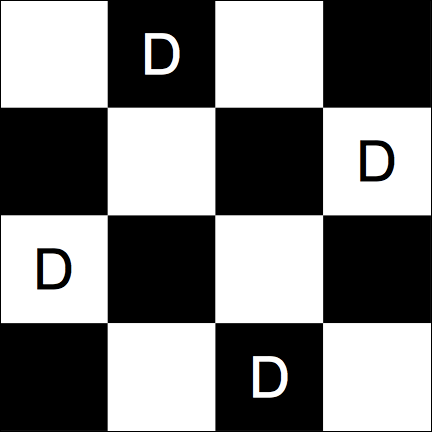
\includegraphics[scale=0.5]{img/four-queens}
	\end{center}
	\caption{\label{four-queens} Lösung des Damenproblems für $n = 4$: In einem Zug kann keine Dame eine andere schlagen.}
\end{figure}

Die Forderung lautet auf einem $n \times n$ großem Schachbrett $n$ Damen so zu platzieren, dass keine Dame eine andere in einem Zug schlagen kann. Abbildung \ref{four-queens} zeigt eine mögliche Lösung.

Zum Testen wurden zwei verschiedene Formeln verwendet. Einerseits ist dies eine handgeschrieben Lösung für $n = 4$, welche Implikationen enthält und dadurch nicht mit minimalen Grammatiken geparst werden kann. Andererseits ist es eine Lösung für $n = 8$ welche mit Hilfe von eigens dafür geschriebenen Funktionen erzeugt wurde. Sie besteht ausschließlich aus den Basisoperatoren Konjunktion, Disjunktion und Negation und ist zudem eine \emph{konjunktive Normalform (KNF bzw. CNF)}.

\subsection{Kartenfärbung USA}

Man stelle sich eine Landkarte der USA mit eingezeichneten Staatsgrenzen vor. Jeder Staat soll nun eingefärbt werden, wobei keine zwei angrenzenden Staaten dieselbe Farbe erhalten dürfen. Diese Aufgabe soll nun mit möglichst wenigen Farben gelöst werden.

Erstellt man eine Formel, welche sämtliche Bedingungen enthält, so kann man das Problem mit einem SAT--Solver lösen. Zur Konstruktion der Formel sei auf \cite{mpa-logeleien} verwiesen.

So kann z. B. gezeigt werden, dass sich eine Karte der USA nicht mit drei Farben kolorieren lässt, jedoch mit vier Farben. Um eine größere Formel zu erhalten, wurde die für vier Farben verwendet. Sie ist in CNF dargestellt.

\subsection{Sudoku}

Dieses ebenfalls aus dem MPA--Projekt stammende Beispiel befasst sich mit dem Sudoku--Spiel. Drückt man die Regeln logisch aus und gibt einige Feldbelegungen vor, so kann das Rätsel wiederum durch einen SAT--Solver gelöst werden. Da eine gültige Belegung hier jedoch irrelevant ist, wurden lediglich die Regeln zum Test benutzt. Sie liegen in CNF vor.

Gemäß Tabelle \ref{formeln-zahlen} wird deutlich, dass die entsprechende Formel signifikant größer als die anderen ist, wodurch die Unzulänglichkeit von Instaparse ursprünglich festgestellt wurde. Um dennoch Messergebnisse eben jenes Parsers erhalten zu können, wurde die Formel zweimal (ungefähr) halbiert. Freilich sind die Regeln dadurch unvollständig geworden, jedoch ist dies hier nicht von Interesse.

\begin{table}[h]
	\begin{tabular}{|l|r|r|r|c|}
		\hline
		\textbf{Name} & \textbf{Anz. Var.} & \textbf{Anz. Op.} & \textbf{Anz. Zeichen} & \textbf{min. Grammatik} \\ \hline
		4--Damen & 200 & 215 & 711 & nein \\ \hline
		8--Damen & 1520 & 2975 & 7487 & ja \\ \hline
		Kartenf. USA & 1608 & 3019 & 16979 & ja \\ \hline
		$^1/_4$ Sudoku & 5832 & 11015 & 40103 & ja \\ \hline
		$^1/_2$ Sudoku & 12393 & 24056 & 86102 & ja \\ \hline
		Sudoku & 24057 & 47384 & 168074 & ja \\ \hline
	\end{tabular}
	\caption{Die zum Test verwendeten Formeln mit den Anzahlen der Variablen, Operatoren, Zeichen und ob die Formel mit einer minimalen Grammatik geparst werden kann.}
	\label{formeln-zahlen}
\end{table}

\section{Messungen}

Gemäß oben genannten Vorgaben wurden nun die Messungen durchgeführt. Die gemittelten Ergebnisse sind in Tabelle \ref{messergebnisse-kurz} einsehbar; die vollständige Messreihe findet sich in \ref{Messergebnisse}.

\begin{table}[h]
	\begin{tabular}{|l|r|r|r|r|r|}
		\hline
		\textbf{Formel} & \textbf{Instaparse \emph{m}} & \textbf{Instaparse. \emph{v}} & \textbf{Kern \emph{m}} & \textbf{Kern \emph{v}} & \textbf{JavaCC} \\ \hline
		\textbf{4--Damen} & - & 111 & - & 180 & 10 \\ \hline
		\textbf{8--Damen} & 354 & 2301 & 293 & 590 & 93 \\ \hline
		\textbf{Kartenf. USA} & 629 & 3890 & 718 & 664 & 204 \\ \hline
		\textbf{$^1/_4$ Sudoku} & 2832 & 25546 & 1282 & 1704 & 461 \\ \hline
		\textbf{$^1/_2$ Sudoku} & 5161 & \textbf{Fehler} & 1643 & 3586 & 524 \\ \hline
		\textbf{Sudoku} & 18361 & \textbf{Fehler} & 3035 & 6894 & 963 \\ \hline 
	\end{tabular}
	\label{messergebnisse-kurz}
	\caption{Messergebnisse im Mittel in Millisekunden. \emph{m} und \emph{v} stehen für \glqq{}minimale\grqq{} und \glqq{}vollständige Grammatik\grqq.}
\end{table}

Ausgeführt wurden die Tests auf einem Asus Zenbook UX31A mit folgender Spezifikation:

\begin{itemize}
	\item Intel Core i7--3517U (4 x 1,9 GHz)
	\item 4 GB RAM
	\item Windows 7 (64 Bit)
	\item Java 1.7.0\_09 (64 Bit)
	\item Clojure 1.5.1
	\item Instaparse 1.2.4
	\item Kern 0.7.0
	\item JavaCC 4.0
\end{itemize}

Das Parsen der halben und der kompletten Sudoku--Regeln mittels der vollständigen Grammatik war mit Instaparse nicht möglich, da es zu einem Stack--Overflow--Fehler geführt hat.

\chapter{Bewertung}

In diesem letzten Abschnitt sollen die erhaltenen Messergebnisse nun analysiert und bewertet werden.

\section{Beobachtungen}

Betrachtet man die Ergebnisse aus Tabelle \ref{messergebnisse-kurz}, so kann man folgende Beobachtungen machen:

\begin{enumerate}
	\item JavaCC benötigt immer und deutlich die wenigste Zeit.
	\item Die Parser mit den vollständigen Grammatiken sind langsamer als die minimalen Grammatiken (Ausnahme: Kern, Kartenfärbung).
	\item Ab einer bestimmten Größe ist der vollständige Kern--Parser schneller als Instaparse mit der Minimalgrammatik.
	\item Die Kern--Parser sind im Allgemeinen schneller als die entsprechneden Instaparse--Produktionen.
	\item Die Laufzeiten von Instaparse wachsen signifikant überproportional zur Größe der Formel.
	\item Nur bei Instaparse treten bei großen Formeln Fehler (Stack Overflow) auf.
\end{enumerate}

Aus 1. folgt, dass der JavaCC--Parser letztendlich in LW eingesetzt wird. Punkt 2. entspricht den Erwartungen.

Die Beobachtungen 3. und 4. weisen darauf hin, dass die Kern--Bibliothek allgemein performanter arbeitet als Instaparse. Es entseht die Frage, ob ein Combinator--Parser grundsätzlich schneller ist als der GLL--Algorithmus, mit dem Instaparse arbeitet \cite[Special Thanks]{instaparse}. Diese Untersuchung ist jedoch nicht Gegenstand dieses Berichts.

Die letzten Punkte (5. und 6.) zeigen hinreichend, dass Instaparse nicht produktiv in LW eingesetzt werden kann. Die generierten Parser sind einfach unzulänglich.

\section{Analyse des Wachstums}

Zwischen den Messergebnissen lassen sich Verhältnisse herstellen, wodurch ein das Wachstum beschreibender Faktor näherungsweise errechnet werden kann. Dies soll in den folgenden Abschnitten geschehen. Für Instaparse gibt es dazu noch eine zusätlich Überlegung, welche vom Autor Mark Engelbert selber stammt. Diese soll mit den hier gemachten Beobachtungen verglichen werden.

Allgemein ist zu beachten, dass die Garbage Collection der JVM eine Rolle spielt, da sie die Laufzeiten signifikant beeinflussen kann. Da die Bedingungen für alle Parser gleich sind und es stark davon abhängt, wie viel \glqq{}Garbage\grqq{} ein Programm produziert, wird dieser Faktor nicht näher betrachtet oder gar herausgerechnet.

\subsection{Engelberts Rechnung zum Instaparse--Wachstum}\label{Engelberg}

Zur Geschwindigkeit von Instaparse hat sich dessen Autor \emph{Mark Engelberg} in der zugehörigen Google--Group zu unserer Problemstellung geäußert. Seine Antwort wird im Folgenden erläutert. \cite{instaparse-google-group}

Es ist festgestellt worden, dass die Grammatik gut konstruiert wurde und die enorm lange Parse--Zeit nicht von Mehrdeutigkeiten in der Grammatik abhinge. Daher bemühte sich Mark Engelberg uns zu helfen, dem Problem auf den Grund zu gehen. Alle hier genannten Messergebnisse gehen auf die Angaben und damit auch den Computer --- von dem wir keine genauere Spezifikation haben --- von Mark Engelberg zurück. Daher können die Messergebnisse auf anderen Rechnern abweichen.

Das angenommene Beispiel waren die vollen Sudokuregeln. Diese sind mit Hilfe von insgesammt 168075 Zeichen (Charactern) beschrieben. Die reine Geschwindigkeit des Lesens wurde duch eine minimale Grammatik geprüft.

\begin{lstlisting}
  S = #'a'+
\end{lstlisting}

Mit dieser Grammatik konnten 168075 Zeichen --- in diesem Fall 168075 \glqq{}a\grqq{} --- innerhalb einer Sekunde geparst werden. Hieraus geht hervor, dass ein starkes Ansteigen der Parse--Zeit eher mit der wachsenden Komplexität der Grammatik zusammenhängt.

Es wurde an dieser Stelle angenommen, dass die Zeit linear zur Komplexität steigt. Wenn also die Grammatik aus 60 Regeln besteht --- wie etwa die volle Grammatik des Parsers für die LW --- sollte das Parsen mit dieser Annahme etwa eine Minute dauern.

Um diese Annahme zu überprüfen, wurde eine Funktion \emph{produce} geschrieben, mit der verschieden große Formeln produziert werden können. Diese haben eine ähnliche Struktur wie die Sudoku--Regeln, wodurch die Laufzeiten des Parsers mit der vollen Grammatik schrittweise im Kleinen überprüft werden können:

\begin{lstlisting}
  (defn ^:dynamic produce [n]
    (cond
      (zero? n) "c1"
      :else (str "(" (produce (dec n)) ")" "&" "(" (produce (dec n)) ")")))

  (def produce (memoize produce))
\end{lstlisting}

\begin{lstlisting}
  => (produce 1)
  "(c1)&(c1)"

  => (produce 2)
  "((c1)&(c1))&((c1)&(c1))"
\end{lstlisting}

Diese Funktion produziert also eine Ausgabe, die immer etwa doppelt so groß wird, wenn man das Argument um eins erhöht:

\begin{lstlisting}
  => (count (produce 14))
  114683

  => (count (produce 15))
  229371
\end{lstlisting}

Wir wollen also einen String parsen, der mit der ungefähren Länge zwischen den Ausgaben von \lstinline|(produce 14)| und \lstinline|(produce 15)| liegt.

Nun betrachten wir die Laufzeit, wenn die Zeichenkette auf die doppelte Länge wächst:

\begin{lstlisting}
  => (time (def x (formula-parser (produce 5))))
  "Elapsed time: 55.882633 msecs"

  => (time (def x (formula-parser (produce 6))))
  "Elapsed time: 104.751713 msecs"

  => (time (def x (formula-parser (produce 7))))
  "Elapsed time: 195.774887 msecs"

  => (time (def x (formula-parser (produce 8))))
  "Elapsed time: 558.543622 msecs"

  => (time (def x (formula-parser (produce 9))))
  "Elapsed time: 1284.250435 msecs"

  => (time (def x (formula-parser (produce 10))))
  "Elapsed time: 2007.042944 msecs"
\end{lstlisting}

Wie man sehen kann, beansprucht das Parsen einer längeren Zeichenkette mehr Zeit. Wenn die Länge der zu parsende Zeichenkette verdoppelt wird, benötigt der Parser etwa doppelt so lange. Die Abweichungen können auf das Eingreifen der Garbage--Collection zurückgeführt werden.

Hierbei ist erkennbar, dass Instaparse mit der hier benutzten Grammatik ein akzeptables Verhalten an den Tag legt. Es ist demzufolge nichts verkehrt an der genutzten Grammatik und die Zeit des Parsens wächs linear proportional zur Eingabegröße. Alles in allem eigentlich ein gutes Ergebnis. Der produzierte Parser hat kein abwegiges Wachstum wie etwa Exponentiel.

Um die den Sudoku--Regeln gleichwertige Eingabegröße zu erreichen, müssen wir die hier vorhandene Formel aus \lstinline|(produce 10)| noch etwa fünfmal verdoppeln. Nach dieser Rechnung sollte der Parser also etwa eine Minute brauchen, um eine Formel der geforderten Eingabegröße zu Parsen.

Theoretisch --- in der Praxis sieht das anders aus. Bei dem Versuch eine Formel von \lstinline|(produce 13)| fängt die Garbage--Collection an zu arbeiten und stört damit massiv den Ablauf. Durch dieses Verhalten verlängert sich die Zeit, die zum Parsen benötigt wird, ungemein. Wobei es in dieser Größenordnung der Eingabe schon teilweise zu Out-Of-Memory-Errors kommt.

%\newpage %sonst ist der nächste Satz von den Punkten abgeschnitten

An dieser Stelle können wir also schon einige Punkte festhalten:

\begin{enumerate}
	\item Im Idealfall braucht Instaparse mit der gegebenen Grammatik etwa eine Minute zum Parsen der gesamten Sudoku--Regeln. Da dies nicht für unseren Anwendungsfall praktikabel war, mussten wir uns nach anderen Möglichkeiten umsehen
	\item Die Praxis zeigt, dass der limitierende Faktor der Arbeitsspeicher ist.
\end{enumerate}

Wir wollen uns nun dem Faktor Arbeitsspeicher widmen. Im Versuchsaufbau konnte mit 1 GB allokiertem Speicher bis zu einer Eingabegröße von \lstinline|(produce 12)| gearbeitet werden, bevor Probleme auftraten. Man kann annehmen, dass Instaparse die Formel für \lstinline|(produce 15)| innerhalb einer Minute parsen kann, wenn man 8 GB Arbeitsspeicher (dreimalige Verdopplung) dafür allokiert --- Diese Theorie wurde von Mark Engelnberg nicht getestet, da er seinen Angaben nach keine einfache Möglichkeit hatte, dies auszuprobieren.\\

Auch mit dieser Annahme wurde gezeigt, dass der aktuelle Instaparse (v 1.2.4) nicht für unsere Anwendung geeignet ist. Das Programm soll ermöglichen, logische Formeln in akzeptabler Zeit zu Parsen. Zum Parsen einer Eingabegröße der Sudoku--Regeln kann man annehmen, dass etwa 8 GB Arbeitsspeicher auschließlich für die Verarbeitung zur Verfügung stehen müssten. Diese Größenordnung ist für die aktuellen Rechner (noch) unüblich. Aber selbst wenn man einen Rechner mit genügent Arbeitsspeicher hat, bräuchte dieser immerhin noch etwa eine Minute zum Parsen. Dies ist im Vergleich zu den hier betrachteten Alternativen ein riesiger Unterschied.

\subsection{Das Verhältnis der gegebenen Formeln}

Zuallererst betrachten wir die Größe der Variablen. Bei dem 4-- und 8--Damen--Problem bestehen die Variablen aus zwei Zeichen. Für die Kartenfärbung werden im Schnitt 7,5 Zeichen pro Variable benötigt und für die Sudoku--Regeln drei.\\

Operatoren als Symbole (also z. B. \glqq{}\&\grqq{} statt \glqq{}and\grqq{}) bestehen im Normalfall aus einem Zeichen. Eine Ausnahme besteht hier bei dem 4--Damen--Problem. Dieses enthält auch den Operator \lstinline|->|. Aus diesem Grund kann diese Formel auch nicht mit der Minimalgrammatik übersetzt werden.\\ % TODO Das hört sich so an, als könnte man 4-Damen nicht machen, weil der Operator zwei Zeichen hat, aber es liegt ja daran, dass es die Regeln in der Minimalgrammatik einfach nicht gibt?

Nun wollen wir den Anstieg der Anzahl der jeweiligen Variablen, Operatoren und Zeichen betrachten.

Das 4--Damen--Problem benötigt 200 Variablen, 215 Operatoren und insgesammt 711 Zeichen. Beim 8--Damen--Problem verzehnfacht sich etwa die Anzahl der Zeichen. Die Anzahl der Variablen ist hierbei um das 7,5--fache angestiegen und die Anzahl der Operatoren sogar um das 15--fache.

Für die Kartenfärbung der USA benötigen wir etwa genauso viele Variablen und Operatoren wie für das 8--Damen--Problem. Da in diesem Fall jedoch die Variablen fast viermal so lang sind, steigt die Zeichenanzahl auf mehr als das Doppelte an. Dieses Verhältnis kann zur Beobachtung genutzt werden, ob die Parse--Zeit eher von der Anzahl der Zeichen oder der Anzahl der Variablen und Operatoren abhängt.

Da die Länge der Variablen zwischen dem 8--Damen-Problem und den Sudoku--Regeln weniger schwanken als bei der Kartenfärbung der USA, vergleichen wir die $^1/_4$ Sudoku--Regeln mit dem 8--Damen--Problem. Dabei vervierfacht sich fast die Anzahl der Variablen und Operatoren, wobei die Anzahl der Zeichen sich mehr als verfünffacht. Dieser unterschiedliche Anstieg von Variablen/Operatoren zu Zeichen kommt daher, dass die Sudokuregeln durch Klammerung starkt geschachtelt sind.

Entsprechend der Abstufungen enthalten die $^1/_2$ Sudoku--Regeln doppelt so viele Variablen, Operatoren und Zeichen. Diese Verdopplung geschieht nocheinmal beim Schritt auf die vollen Sudoku--Regeln.

\subsection{Instaparse}

Nun wollen wir das Wachstum der Parse--Zeit für Instaparse im Zusammenhang mit der Eingabe betrachten.

Für das 4--Damen--Problem braucht der \emph{Instaparse--Parser mit der vollen Grammatk (IPv)} 111 ms. Das diese Formel mit der Minimalgrammatik nicht zu parsen war, liegt in diesem Fall keine Zeit für den \emph{Instaparse--Parser mit der minimalen Grammatk (IPm)} vor.

Für das 8--Damen--Probmlem brauchte der IPm 354 ms und der IPv 2301 ms. Für dem IPv ist das mehr als die zwanzigfache Zeit. Dies fällt in etwa in die Größenordnung vom Anstieg der Variablen und Zeichen.

Der IPm braucht 629 ms und der IPv 3890 ms zum Parsen der Kartenfärbung der USA. In beiden Fällen ist das fast eine Verdopplung der Zeit. Da die Anzahl der Variablen und Operatoren gleich geblieben ist, kann man hier annehmen, dass sich dies auf die Erhöhung der Zeichen auf etwas mehr als das Doppelte der Parse--Zeit auswirkt.

Für das Parsen der $^1/_4$ Sudoku--Regeln braucht der IPm achtmal und der IPv etwa elfmal so lange wie für das 8--Damen--Problem. Man kann daher annehmen, dass das Parsen mit dem Instaparse--Parser durch die starke Verschachtelung mittels Klammern die Parse--Zeit steigert. Hierbei kann der Unterschied zwischen der Erhöhung zwischen IPm und IPv daran liegen, dass die Klammer--Regel sehr weit unten in der Grammatik beschrieben ist, wobei die minimale Grammatik weniger Regeln hat, die bis zur Klammerungsregel geprüft werden müssen. Des Weiteren ist anzunehmen, dass beim IPv die Garbage Collection einsetzt und sich dies negativ auf die Zeit auswirkt.

Wie in der Beschreibung von Mark Engelberg (siehe Abschnitt \ref{Engelberg}) angenommen und gezeigt wurde, hat sich die Parse--Zeit für IPm von $^1/_4$ zu $^1/_2$ Sudoku--Regeln verdoppelt. Der IPv konnte die $^1/_2$ Sudoku--Regeln nicht mehr Parsen, da es dabei immer wieder zu Fehlern (\emph{OutOfMemoryException, StackOverflowError, ...}) kam.

Die benötigte Zeit vervierfacht sich fast zum Parsen der gesamten Sudokuregel. Hier ist zu erkennen, dass sich die Garbage Collection massiv auf die benötigte Zeit auswirkt.\\

Nun betrachten wir das Zeitverhältnis zwischen IPm und IPv. Zu Anfang lässt sich annehmen, dass der IPv etwa sechsmal länger braucht als der IPm. Beim Parsen der $^1/_4$ Sudoku--Regeln dauert es aber etwa zehnmal so lange. Wir nehmen also an, dass es sich um ein exponentielles Verhältnis ($x^n$) handelt. Hierbei konnte ermittelt werden, dass der Exponent ($^n$) bei etwa 1,293 liegt. Mit Hilfe diese Annahme wurden die theoretischen Werte für den IPv und den IPm errechnet.

\subsection{Kern}
%TODO
\subsection{JavaCC}
%TODO

\appendix

\begin{thebibliography}{7}
	\bibitem[LW]{lw}
		Quellcode des Projektes auf Github, 
		\url{https://github.com/moerkb/logical-workbench}

	\bibitem[LWFORM]{lw-formeln}
		Testformeln,
		\url{https://github.com/moerkb/logical-workbench/blob/master/src/parser_measures/formulas.clj}

	\bibitem[KERN]{kern}
		Armando Blancas,
		Projektseite der Bibliothek Kern, 
		\url{https://github.com/blancas/kern}

	\bibitem[INSTA]{instaparse}
		Mark Engelberg,
		Projektseite der Bibliothek Instaparse,
		\url{https://github.com/Engelberg/instaparse}

	\bibitem[JAVACC]{javacc}
		Java Compiler Compiler,
		\url{https://javacc.java.net}

	\bibitem[MPA]{mpa}
		Prof. Dr. B. Renz,
		Projektseite des MPA,
		\url{http://homepages.thm.de/~hg11260/mpa.html}

	\bibitem[INSTGR]{instaparse-google-group}
		Diskussion über Instaparse--Laufzeiten mit Autor Mark Engelberg, 
		\url{https://groups.google.com/forum/#!topic/instaparse/GYoswP-X7O8}

	\bibitem[MPALOG]{mpa-logeleien}
		Prof. Dr. B. Renz,
		Lösungen mit dem MNI Proposition Analyzer MPA --- Logeleien, Kartenfärbung, Sudoku, Variabilitätsmodelle,
		\url{http://homepages.thm.de/~hg11260/mat/mpa-bsp.pdf}
\end{thebibliography}

\clearpage
\begingroup
\let\clearpage\relax
\listoffigures
\listoftables
\endgroup

\chapter{Sonstiges}
\section{Messergebnisse}
\begin{table}[!h]
	\resizebox{!}{\textwidth}{
		\rotatebox{90}{
			\begin{tabular}{|l|r|r|r|r|r|r|r|r|r|r|r|}
				\hline
				\textbf{4 Damen} & \multicolumn{1}{l|}{} & \multicolumn{1}{l|}{} & \multicolumn{1}{l|}{} & \multicolumn{1}{l|}{} & \multicolumn{1}{l|}{} & \multicolumn{1}{l|}{} & \multicolumn{1}{l|}{} & \multicolumn{1}{l|}{} & \multicolumn{1}{l|}{} & \multicolumn{1}{l|}{} & \multicolumn{1}{l|}{} \\ \hline
				javacc  & 10 & 9 & 10 & 8 & 7 & 15 & 11 & 9 & 15 & 10 & 10 \\ \hline
				kern, voll   & 199 & 199 & 191 & 190 & 187 & 186 & 54 & 194 & 201 & 196 & 180 \\ \hline
				instaparse, minimal   & \multicolumn{1}{l|}{} & \multicolumn{1}{l|}{} & \multicolumn{1}{l|}{} & \multicolumn{1}{l|}{} & \multicolumn{1}{l|}{} & \multicolumn{1}{l|}{} & \multicolumn{1}{l|}{} & \multicolumn{1}{l|}{} & \multicolumn{1}{l|}{} & \multicolumn{1}{l|}{} & (38) \\ \hline
				instaparse, voll   & 118 & 110 & 107 & 110 & 108 & 121 & 108 & 109 & 112 & 108 & 111 \\ \hline
				\textbf{8 Damen} & \multicolumn{1}{l|}{} & \multicolumn{1}{l|}{} & \multicolumn{1}{l|}{} & \multicolumn{1}{l|}{} & \multicolumn{1}{l|}{} & \multicolumn{1}{l|}{} & \multicolumn{1}{l|}{} & \multicolumn{1}{l|}{} & \multicolumn{1}{l|}{} & \multicolumn{1}{l|}{} & \multicolumn{1}{l|}{} \\ \hline
				javacc  & 92 & 94 & 94 & 72 & 90 & 104 & 93 & 98 & 88 & 109 & 93 \\ \hline
				kern, minimal   & 285 & 276 & 292 & 296 & 275 & 279 & 371 & 286 & 287 & 287 & 293 \\ \hline
				kern, voll   & 645 & 624 & 567 & 649 & 570 & 563 & 468 & 551 & 638 & 626 & 590 \\ \hline
				instaparse, minimal   & 298 & 369 & 345 & 291 & 366 & 376 & 348 & 355 & 368 & 419 & 354 \\ \hline
				instaparse, voll   & 2351 & 2223 & 2249 & 2277 & 2330 & 2306 & 2730 & 2328 & 2238 & 1975 & 2301 \\ \hline
				\textbf{USA} & \multicolumn{1}{l|}{\textbf{}} & \multicolumn{1}{l|}{\textbf{}} & \multicolumn{1}{l|}{\textbf{}} & \multicolumn{1}{l|}{\textbf{}} & \multicolumn{1}{l|}{\textbf{}} & \multicolumn{1}{l|}{\textbf{}} & \multicolumn{1}{l|}{\textbf{}} & \multicolumn{1}{l|}{\textbf{}} & \multicolumn{1}{l|}{\textbf{}} & \multicolumn{1}{l|}{\textbf{}} & \textbf{Mittel} \\ \hline
				javacc  & 208 & 217 & 206 & 196 & 179 & 205 & 210 & 212 & 197 & 215 & 204 \\ \hline
				kern, minimal   & 610 & 814 & 832 & 859 & 618 & 593 & 596 & 791 & 851 & 613 & 718 \\ \hline
				kern, voll   & 673 & 665 & 670 & 719 & 658 & 639 & 673 & 660 & 627 & 652 & 664 \\ \hline
				instaparse, minimal   & 595 & 593 & 584 & 607 & 998 & 590 & 553 & 609 & 572 & 592 & 629 \\ \hline
				instaparse, voll   & 4094 & 3652 & 3649 & 3607 & 3798 & 4386 & 4141 & 3759 & 3769 & 4040 & 3890 \\ \hline
				\textbf{Viertel Sudoku} & \multicolumn{1}{l|}{} & \multicolumn{1}{l|}{} & \multicolumn{1}{l|}{} & \multicolumn{1}{l|}{} & \multicolumn{1}{l|}{} & \multicolumn{1}{l|}{} & \multicolumn{1}{l|}{} & \multicolumn{1}{l|}{} & \multicolumn{1}{l|}{} & \multicolumn{1}{l|}{} & \multicolumn{1}{l|}{} \\ \hline
				javacc  & 629 & 379 & 393 & 375 & 380 & 375 & 659 & 651 & 383 & 384 & 461 \\ \hline
				kern, minimal   & 1274 & 1290 & 1251 & 1292 & 1245 & 1262 & 1345 & 1289 & 1287 & 1283 & 1282 \\ \hline
				kern, voll   & 1720 & 1686 & 1676 & 1792 & 1617 & 1714 & 1707 & 1710 & 1745 & 1670 & 1704 \\ \hline
				instaparse, minimal   & 2102 & 2434 & 3939 & 2322 & 3655 & 2566 & 2096 & 2017 & 3506 & 3686 & 2832 \\ \hline
				instaparse, voll   & 31108 & 28401 & 21306 & 21629 & 21233 & 20991 & 28230 & 28365 & 29472 & 24725 & 25546 \\ \hline
				\textbf{Halbes Sudoku} & \multicolumn{1}{l|}{} & \multicolumn{1}{l|}{} & \multicolumn{1}{l|}{} & \multicolumn{1}{l|}{} & \multicolumn{1}{l|}{} & \multicolumn{1}{l|}{} & \multicolumn{1}{l|}{} & \multicolumn{1}{l|}{} & \multicolumn{1}{l|}{} & \multicolumn{1}{l|}{} & \multicolumn{1}{l|}{} \\ \hline
				javacc  & 472 & 483 & 580 & 489 & 626 & 552 & 419 & 570 & 443 & 609 & 524 \\ \hline
				kern, minimal   & 1657 & 1606 & 1628 & 1714 & 1646 & 1616 & 1706 & 1659 & 1604 & 1591 & 1643 \\ \hline
				kern, voll   & 3580 & 3473 & 3557 & 3741 & 3589 & 3484 & 3735 & 3651 & 3513 & 3535 & 3586 \\ \hline
				instaparse, minimal   & 5151 & 4708 & 5085 & 4941 & 5714 & 4698 & 4196 & 4913 & 5270 & 6938 & 5161 \\ \hline
				instaparse, voll   & \multicolumn{1}{l|}{} & \multicolumn{1}{l|}{} & \multicolumn{1}{l|}{} & \multicolumn{1}{l|}{} & \multicolumn{1}{l|}{} & \multicolumn{1}{l|}{} & \multicolumn{1}{l|}{} & \multicolumn{1}{l|}{} & \multicolumn{1}{l|}{} & \multicolumn{1}{l|}{} & (63184) \\ \hline
				\textbf{Sudoku} & \multicolumn{1}{l|}{} & \multicolumn{1}{l|}{} & \multicolumn{1}{l|}{} & \multicolumn{1}{l|}{} & \multicolumn{1}{l|}{} & \multicolumn{1}{l|}{} & \multicolumn{1}{l|}{} & \multicolumn{1}{l|}{} & \multicolumn{1}{l|}{} & \multicolumn{1}{l|}{} & \multicolumn{1}{l|}{} \\ \hline
				javacc  & 695 & 1182 & 1028 & 1044 & 1091 & 670 & 720 & 1101 & 1031 & 1067 & 963 \\ \hline
				kern, minimal   & 3051 & 2941 & 3014 & 3198 & 2996 & 2991 & 3141 & 3064 & 2967 & 2982 & 3035 \\ \hline
				kern, voll   & 6977 & 6631 & 6777 & 7279 & 6806 & 6669 & 7165 & 7054 & 6726 & 6852 & 6894 \\ \hline
				instaparse, minimal   & 19072 & 18782 & 18530 & 18439 & 17480 & 19001 & 19870 & 18148 & 18547 & 15740 & 18361 \\ \hline
				instaparse, voll   & \multicolumn{1}{l|}{} & \multicolumn{1}{l|}{} & \multicolumn{1}{l|}{} & \multicolumn{1}{l|}{} & \multicolumn{1}{l|}{} & \multicolumn{1}{l|}{} & \multicolumn{1}{l|}{} & \multicolumn{1}{l|}{} & \multicolumn{1}{l|}{} & \multicolumn{1}{l|}{} & (325998) \\ \hline
				\end{tabular}
			}
		}
		\label{Messergebnisse}
		\caption{Ergebnisse der Messreihen, alle Angaben in Millisekunden. Ergebnisse in Klammern sind errechnet.}
\end{table}

\newpage
\section{Referenzgrammatik}\label{refgrammatik}

Das folgende Listing stammt aus der Hilfe--Datei des MPA. \cite{mpa}

\begin{verbatim}	
Proposition	::=	Atom | Const
| "(" UnOp Proposition ")"
| "(" Proposition BinOp Proposition ")"
Atom	::=	([letter]|"_"|"\"|"{"|"}")([letter]|[digit]|"_"|"\"|"{"|"}")*
Const	::=	("T"|"1"|"True"|"F"|"0"|"False")
UnOp	::=	("!"|"not")
BinOp	::=	see Section below
\end{verbatim}

Formeln können mit runden ( (\dots) ) oder eckigen Klammern ( [\dots] ) zusammengefasst werden. Kommentare sind mit (//\dots) zeilenweise oder durch (/*\dots */) blockweise möglich.

Die binären Operatoren \glqq{}BinOp\grqq{} sind wie folgt organisiert:

\begin{table}[h]
	\begin{tabular}{|l|l|l|}
		\hline
		\textbf{Beschreibung} & \textbf{Syntax} & \textbf{Assoziativität} \\
		\hline
		Und & \&, and & links \\ \hline
		Nicht--Und & !\&, nand & links \\ \hline
		Oder & |, or & links \\ \hline
		Nicht--Oder & !|, nor & links \\ \hline
		Rechtsimplikation & <-, if & rechts \\ \hline
		negierte Rechtsimplikation & nif & rechts \\ \hline
		Implikation & ->, impl & rechts \\ \hline
		negierte Implikation & nimpl & rechts \\ \hline
		Äquivalenz & <->, iff & links \\ \hline
		exklusives Oder & \textasciicircum, xor & links \\ \hline
	\end{tabular}
	\caption{Binäroperatoren mit Syntax und Assoziativität, absteigend sortiert nach Präzedenz}
\end{table}

\end{document}
